\\
\documentclass{beamer}
\usetheme{CambridgeUS}
\title{Tyre Inspection and Analysis Using Deep Learning}
\author{Ebin Joseph\inst{1} \and Ebin Sebastian\inst{2} \and Arun A S\inst{3} \and \\ Project Guide: Dr. Rajeswari M}

\institute[Sahrdaya College of Engineering and Technology] 
{
  Department of Computer Science\\
  Sahrdaya College of Engineering and Technology
 }

\date{First Project Review, 2019}
\subject{Tyre Inspection and Analysis Using Deep Learning}
\AtBeginSubsection[]
{
  \begin{frame}<beamer>{Outline}
    \tableofcontents[currentsection,currentsubsection]
  \end{frame}
}

\begin{document}

\begin{frame}
  \titlepage
\end{frame}

\begin{frame}{Outline}
  \tableofcontents[pausesections]
  % You might wish to add the option [pausesections]
\end{frame}

\section{Introduction}
\subsection*{}
\begin{frame}{Introduction}
\begin{block}{}
In this project, we create a mobile application which is able to predict the durability of tyre and the damages occured to it.
\end{block}
\end{frame}

\section{Objectives}
\subsection*{}
\begin{frame}{Objectives}
\begin{itemize}
\item{Collect Data}
\item{Design neural network architecture}
\item{Train network}
\item{Validate the trained network}
\item{Optimize network}
\item{Deploy in a mobile platform}
\end{itemize}
\end{frame}


\section{Proposed Plan}
\subsection*{}
\begin{frame}{Proposed Plan}
\begin{itemize}
\item{
It is hard to approach organizations with out a working prototype
}
\end{itemize}
\end{frame}
\subsection*{}
\begin{frame}{Proposed Plan}
\begin{itemize}
\item{
It is hard to approach organizations with out a working prototype
\begin{itemize}
\item{
Create a mock data-set by taking pictures and downloading pictures from web.
}
\end{itemize}
}
\end{itemize}
\end{frame}
\subsection*{}
\begin{frame}{Proposed Plan}
\begin{itemize}
\item{
It is hard to approach organizations with out a working prototype
\begin{itemize}
\item{
Create a mock data-set by taking pictures and downloading pictures from web.
}
\end{itemize}
}
\item{
Design a neural network architecture based on the mock data-set.
}
\end{itemize}
\end{frame}
\subsection*{}
\begin{frame}{Proposed Plan}
\begin{itemize}
\item{
It is hard to approach organizations with out a working prototype
\begin{itemize}
\item{
Create a mock data-set by taking pictures and downloading pictures from web.
}
\end{itemize}
}
\item{
Design a neural network architecture based on the mock data-set.
}
\item{
Optimize the architecture.
}
\end{itemize}
\end{frame}
\subsection*{}
\begin{frame}{Proposed Plan}
\begin{itemize}
\item{
It is hard to approach organizations with out a working prototype
\begin{itemize}
\item{
Create a mock data-set by taking pictures and downloading pictures from web.
}
\end{itemize}
}
\item{
Design a neural network architecture based on the mock data-set.
}
\item{
Optimize the architecture.
}
\item{
create and train the neural network with mock data-set and deploy it to create a working prototype
}
\end{itemize}
\end{frame}
\subsection*{}
\begin{frame}{Proposed Plan}
\begin{itemize}
\item{
It is hard to approach organizations with out a working prototype
\begin{itemize}
\item{
Create a mock data-set by taking pictures and downloading pictures from web.
}
\end{itemize}
}
\item{
Design a neural network architecture based on the mock data-set.
}
\item{
Optimize the architecture.
}
\item{
create and train the neural network with mock data-set and deploy it to create a working prototype
}
\item{
Use the prototype to obtain valid data-sets.
}
\end{itemize}
\end{frame}
\subsection*{}
\begin{frame}{Proposed Plan}
\begin{itemize}
\item{
It is hard to approach organizations with out a working prototype
\begin{itemize}
\item{
Create a mock data-set by taking pictures and downloading pictures from web.
}
\end{itemize}
}
\item{
Design a neural network architecture based on the mock data-set.
}
\item{
Optimize the architecture.
}
\item{
create and train the neural network with mock data-set and deploy it to create a working prototype
}
\item{
Use the prototype to obtain valid data-sets.
}
\item{
Use the valid data-set to make corresponding changes to the architecture.
}
\end{itemize}
\end{frame}
\subsection*{}
\begin{frame}{Proposed Plan}
\begin{itemize}
\item{
It is hard to approach organizations with out a working prototype
\begin{itemize}
\item{
Create a mock data-set by taking pictures and downloading pictures from web.
}
\end{itemize}
}
\item{
Design a neural network architecture based on the mock data-set.
}
\item{
Optimize the architecture.
}
\item{
create and train the neural network with mock data-set and deploy it to create a working prototype
}
\item{
Use the prototype to obtain valid data-sets.
}
\item{
Use the valid data-set to make corresponding changes to the architecture.
}
\item{
Recreate the neural network and train it.
}
\end{itemize}
\end{frame}
\subsection*{}
\begin{frame}{Proposed Plan}
\begin{itemize}
\item{
It is hard to approach organizations with out a working prototype
\begin{itemize}
\item{
Create a mock data-set by taking pictures and downloading pictures from web.
}
\end{itemize}
}
\item{
Design a neural network architecture based on the mock data-set.
}
\item{
Optimize the architecture.
}
\item{
create and train the neural network with mock data-set and deploy it to create a working prototype
}
\item{
Use the prototype to obtain valid data-sets.
}
\item{
Use the valid data-set to make corresponding changes to the architecture.
}
\item{
Recreate the neural network and train it.
}
\item{
Validate and optimize the network.
}
\end{itemize}
\end{frame}
\subsection*{}
\begin{frame}{Proposed Plan}
\begin{itemize}
\item{
It is hard to approach organizations with out a working prototype
\begin{itemize}
\item{
Create a mock data-set by taking pictures and downloading pictures from web.
}
\end{itemize}
}
\item{
Design a neural network architecture based on the mock data-set.
}
\item{
Optimize the architecture.
}
\item{
create and train the neural network with mock data-set and deploy it to create a working prototype
}
\item{
Use the prototype to obtain valid data-sets.
}
\item{
Use the valid data-set to make corresponding changes to the architecture.
}
\item{
Recreate the neural network and train it.
}
\item{
Validate and optimize the network.
}
\item{
Deploy to Android.
}
\end{itemize}
\end{frame}

\section{Design of Diagrams}

\subsection{Flow Diagram}
\begin{frame}{Flow Diagram}
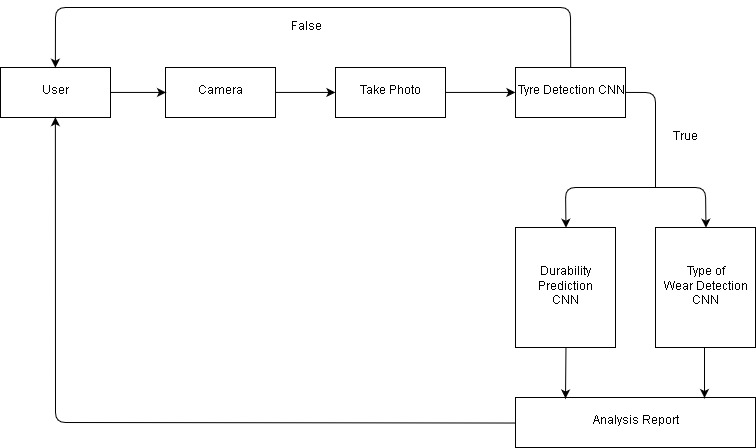
\includegraphics[scale=0.37]{second.jpg}
\end{frame}

\subsection{Neural Network Architectures}
\begin{frame}{Neural Network Architectures}
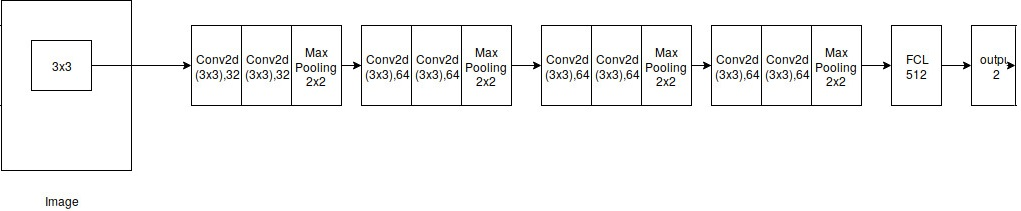
\includegraphics[scale=0.33]{arch.png}
\end{frame}

\section{Algorithms}
\subsection{}
\begin{frame}{Algorithm}
\begin{block}{}
Algorithm: Forward Propagation\\
for k = 1 to L -1\\
\quad \quad $a_{k} = b_{k} + W_{k} H_{k - 1}$\\
\quad \quad $h_{k} = g(a_{k})$\\
end\\
$a_{L} = b_{L} + W_{L}H_{L-1}$\\
$\hat y = O(a_{L})$\\
\quad\\
$L = $ number of layers\\
$a_{k} = $ vector of total sum of $k^{th}$ layer , 
$b_{k} = $ vector of biases of $k^{th}$ layer , 
$W_{k} = $ vector of weights of $k^{th}$ layer , 
$h_{k} = $ vector of outputs of $k^{th}$ layer , 
$g = $ activation function , 
$H_{k-1} = $ vector of Outputs of $(k-1)^{th}$ layer , 
$\hat y = $ output of network , 
$O = $ activation function of output layer.
\end{block}
\end{frame}


\section{Present Status}
\subsection{}
\begin{frame}{Present Status}
\begin{itemize}
\item{Designed system architecture}
\item{Implemented the First neural network}
\item{Old trained model was lost due to version change}
\item{Deployed application on local network}
\item{Attempting to train on Google Colab}
\end{itemize}
\end{frame}


\section{Conclusion}
\subsection{}
\begin{frame}{Conclusion}
\begin{itemize}
\item{More powerful machine is needed for training with larger datasets.}
\item{Due to size limits on free hosting sites, we have temporarily hosted on local network.}

\end{itemize}
\end{frame}


\section{Future Plans}
\subsection{}
\begin{frame}{Future Plans}
\begin{itemize}
\item{Use RNN.}
\item{Sequential detection.}
\item{Multiple network for multiple classes.}
\item{Place backend as REST API.}
\end{itemize}
\end{frame}


\section{Conference Attended}
\subsection{}
\begin{frame}{Conference Attended}
\begin{itemize}
\item{Attended conference ICITIST 2018 in SIST on Nov 27th 2018}

\end{itemize}
\end{frame}



\section{References}
\subsection{}
\begin{frame}{References}
\begin{itemize}
\item{YOLOv3: An Incremental Improvement,Redmon, Joseph and Farhadi, Ali,arXiv,2018}
\item{Generative Adversarial Nets, Ian J. Goodfellow, Jean Pouget-Abadie, arxiv, 2014}
\item{Very Deep Convolutional Networks for Large-Scale Image Recognition, Karen Simonyan, Andrew Zisserman, arxiv, 2015}
\item{Rethinking the Inception Architecture for Computer Vision, Christian Szegedy, Vincent Vahoucke, arxiv, 2015}
\item{Deep Residual Learning for Image Recognition, Kaiming He, Xiangyu Zhang, arxiv, 2015}
\item{Generative Adversarial Nets, Ian J. Goodfellow, Jean Pouget-Abadie, arxiv, 2014}
\item{Aggregated Residual Transformations for Deep Neural Networks, Saining Shi, Ross Girshick, arxiv, 2017}
\item{ImageNet Classification with Deep Convolutional Neural Networks, Alex Krizhevsky, Ilya Sutskever , 2012}





\end{itemize}
\end{frame}
\end{document}


